% generated by scripts/pkl_to_latex.py
% source PKL : vscan_v1_L6_Ne5_U10_t1_mode-uniform_nmin2_solver-gcg_full_restarts10_iter300_kmax4_tol1em09_V0to15_N16-2f7c06936fa2.pkl
% scan type  : vscan
% state      : gs
% requires   : \usepackage{pgfplots} \pgfplotsset{compat=1.18}
% colours match the matplotlib PDF (tab10 cycle)
\definecolor{gmeC0}{HTML}{1F77B4}
\definecolor{gmeC1}{HTML}{FF7F0E}
\definecolor{gmeC2}{HTML}{2CA02C}
\definecolor{gmeC3}{HTML}{D62728}
\definecolor{gmeC4}{HTML}{9467BD}
\definecolor{gmeC5}{HTML}{8C564B}
\definecolor{gmeC6}{HTML}{E377C2}
\definecolor{gmeC7}{HTML}{17BECF}

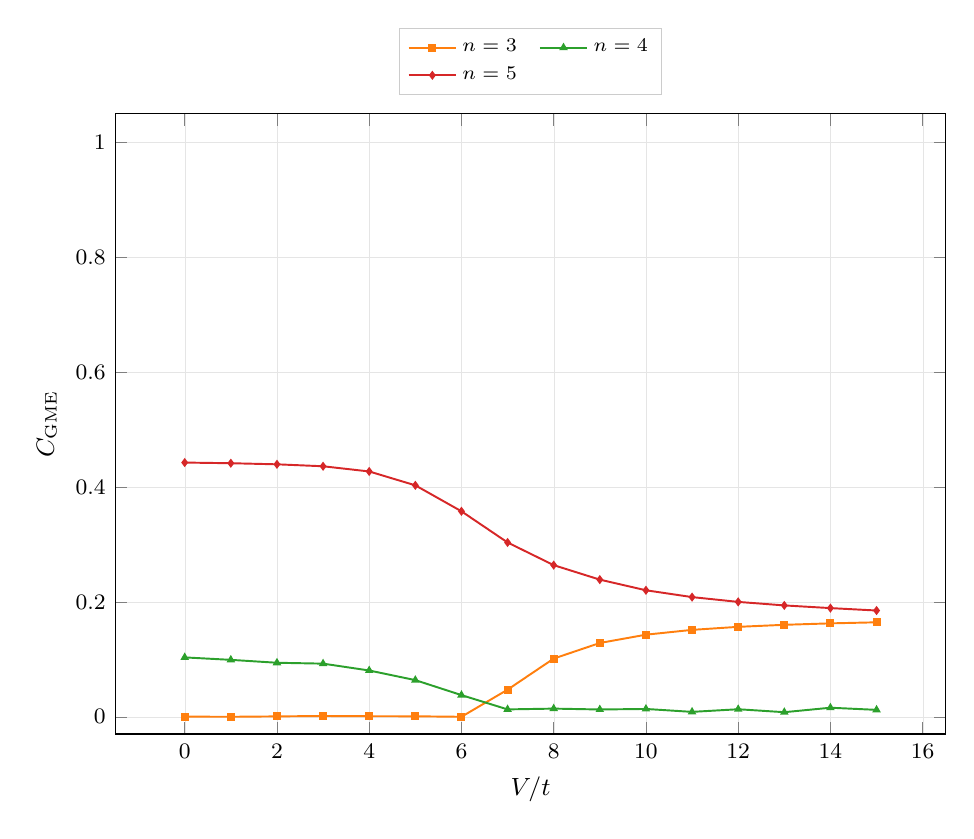
\begin{tikzpicture}
  \begin{axis}[
    width=\columnwidth,
    height=0.78\columnwidth,
    xlabel={$V/t$},
    ylabel={$C_{\mathrm{GME}}$},
    grid=both,
    grid style={line width=.1pt, draw=gray!20},
    tick label style={font=\footnotesize\rmfamily, /pgf/number format/fixed},
    label style={font=\small\rmfamily},
    scaled ticks=false,
    legend style={font=\scriptsize\rmfamily, draw=gray!40, at={(0.5,1.03)}, anchor=south, /tikz/every even column/.append style={column sep=6pt}},
    legend cell align={left},
    legend columns=2,
    ymin=-0.03,
    ymax=1.05,
  ]
    \addplot[color=gmeC1, mark=square*, mark size=1.1pt, line width=0.7pt] coordinates {
        (0,0.000314) (1,0.000028) (2,0.000715) (3,0.001426)
        (4,0.000996) (5,0.000874) (6,0.000029) (7,0.047258)
        (8,0.101385) (9,0.128553) (10,0.142995) (11,0.151389)
        (12,0.156669) (13,0.160213) (14,0.162719) (15,0.164567)
    };
    \addlegendentry{$n=3$}
    \addplot[color=gmeC2, mark=triangle*, mark size=1.1pt, line width=0.7pt] coordinates {
        (0,0.103452) (1,0.099191) (2,0.094114) (3,0.092585)
        (4,0.080651) (5,0.063904) (6,0.037803) (7,0.012908)
        (8,0.014261) (9,0.012754) (10,0.013668) (11,0.008592)
        (12,0.013176) (13,0.00803) (14,0.015821) (15,0.012093)
    };
    \addlegendentry{$n=4$}
    \addplot[color=gmeC3, mark=diamond*, mark size=1.1pt, line width=0.7pt] coordinates {
        (0,0.442751) (1,0.441599) (2,0.439696) (3,0.436306)
        (4,0.427254) (5,0.403108) (6,0.357887) (7,0.303576)
        (8,0.264107) (9,0.238878) (10,0.220358) (11,0.208475)
        (12,0.200112) (13,0.193975) (14,0.189318) (15,0.185095)
    };
    \addlegendentry{$n=5$}
  \end{axis}
\end{tikzpicture}
